\documentclass[10pt]{beamer}
\usetheme[
%%% option passed to the outer theme
%    progressstyle=fixedCircCnt,   % fixedCircCnt, movingCircCnt (moving is deault)
  ]{Feather}
  
% If you want to change the colors of the various elements in the theme, edit and uncomment the following lines

% Change the bar colors:
\setbeamercolor{Feather}{fg=shtred!20,bg=shtred}

% Change the color of the structural elements:
\setbeamercolor{structure}{fg=shtred}

% Change the frame title text color:
%\setbeamercolor{frametitle}{fg=blue}

% Change the normal text color background:
%\setbeamercolor{normal text}{fg=black,bg=gray!10}

%-------------------------------------------------------
% INCLUDE PACKAGES
%-------------------------------------------------------

\usepackage[utf8]{inputenc}
\usepackage[english]{babel}
\usepackage[T1]{fontenc}
\usepackage{helvet}
\usepackage{subcaption}
\usepackage{amsmath}

\makeatletter
\renewcommand*\env@matrix[1][*\c@MaxMatrixCols c]{%
  \hskip -\arraycolsep
  \let\@ifnextchar\new@ifnextchar
  \array{#1}}
\makeatother
%-------------------------------------------------------
% DEFFINING AND REDEFINING COMMANDS
%-------------------------------------------------------

% colored hyperlinks
\newcommand{\chref}[2]{
  \href{#1}{{\usebeamercolor[bg]{Feather}#2}}
}

%-------------------------------------------------------
% INFORMATION IN THE TITLE PAGE
%-------------------------------------------------------

\title[] % [] is optional - is placed on the bottom of the sidebar on every slide
{ % is placed on the title page
      \textbf{Reinforcement Learning - Introduction}
}

\subtitle[ Reinforcement Learning - Introduction ]
{
      \textbf{}
}

\author[Mohit Rathore]
{      Mohit Rathore \\
	mrmohitrathoremr@gmail.com\\
}

\institute[]
{
      Center for Visual Information Technology\\
    IIIT Hyderabad\\
  
  %there must be an empty line above this line - otherwise some unwanted space is added between the university and the country (I do not know why;( )
}

\date{Sep 7, 2018}

%-------------------------------------------------------
% THE BODY OF THE PRESENTATION
%-------------------------------------------------------

\begin{document}

%-------------------------------------------------------
% THE TITLEPAGE
%-------------------------------------------------------

{\1% % this is the name of the PDF file for the background
\begin{frame}[plain,noframenumbering] % the plain option removes the header from the title page, noframenumbering removes the numbering of this frame only
  \titlepage % call the title page information from above
\end{frame}}


\begin{frame}{Contents}{}
\tableofcontents
\end{frame}

%-------------------------------------------------------
\section{Trivia}
%-------------------------------------------------------
\subsection{Motivation}
\begin{frame}{Trivia}{Why should I care?}
%-------------------------------------------------------
  \begin{itemize}
    \item At the very core deep learning can solve problem of classification, regression i.e. approximating complex functions.
    \item Reinforcement learning on the other hand help's us devise an optimum strategy to follow in our feat of maximizing reward.
  \end{itemize}

\begin{figure}[!htb]
\centering
\begin{subfigure}[t]{0.6\linewidth}

\includegraphics[width=.65\textwidth]{assets/adv_ai_meme.jpg}
\end{subfigure}

\vspace{0.1in}
\label{fig:tripEmb}
\end{figure}

\end{frame}

%-------------------------------------------------------
\subsection{News}
\begin{frame}{Trivia}{News}
  \begin{itemize}
    \item RL Beats Humans at Dota 2. \href{https://www.youtube.com/watch?time_continue=4&v=UZHTNBMAfAA}{\beamergotobutton{Link}}
    \item AlphaGo beats 18-time world champion Lee Sedol. \href{https://www.youtube.com/watch?v=l7ngy56GY6k}{\beamergotobutton{Link}}
    \item Google has developed an approach to hyperparameter tuning using reinforcement learning that they call AutoML. \href{https://cloud.google.com/automl/}{\beamergotobutton{Link}}
    
  \end{itemize}
\end{frame}
%-------------------------------------------------------

\section{Deep Q Learning}
%-------------------------------------------------------
\subsection{Understanding the terms.}
\begin{frame}{Introduction}{Jargons}

\begin{itemize}
\item \textbf{State} - It can be seen as a variable which directly affect the action taking mechanism. 
In an environment such as a maze, a state can be seen as the x, y coordinates of the agent.

\end{itemize}

\begin{figure}[!htb]
\centering
\begin{subfigure}[t]{0.6\linewidth}
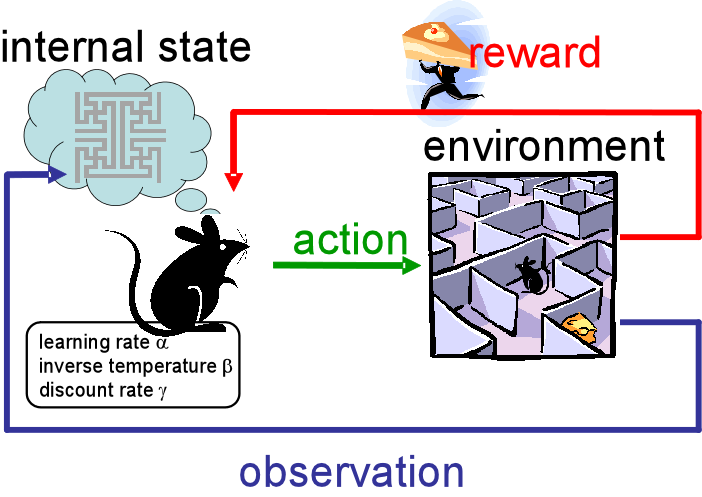
\includegraphics[width=.9\textwidth]{assets/mouserl.png}
\end{subfigure}

\vspace{0.1in}
\label{fig:tripEmb}
\end{figure}

\end{frame}
%-------------------------------------------------------
\begin{frame}{Introduction}{Jargons}

\begin{itemize}
\item \textbf{Action} - Performing a particular action in a particular state takes you to the next state. 
\item The mouse can move in either of the four directions to reach the next block.
\end{itemize}

\begin{figure}[!htb]
\centering
\begin{subfigure}[t]{0.6\linewidth}
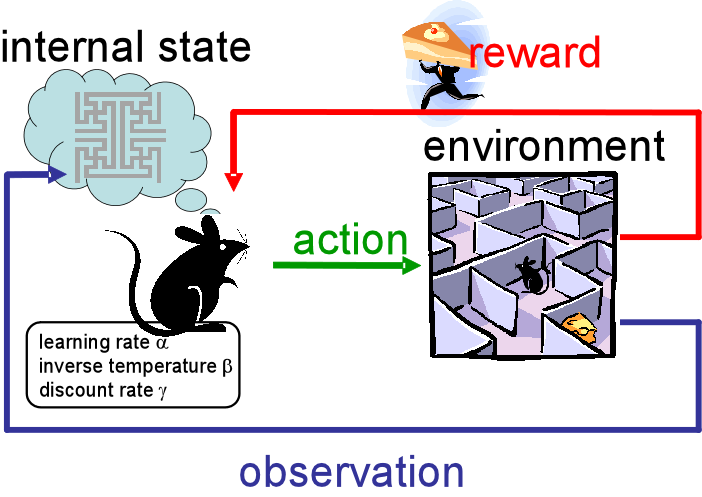
\includegraphics[width=.9\textwidth]{assets/mouserl.png}
\end{subfigure}

\vspace{0.1in}
\label{fig:tripEmb}
\end{figure}

\end{frame}
%-------------------------------------------------------
\begin{frame}{Introduction}{Jargons}

\begin{itemize}
\item \textbf{Agent} - It is an abstraction of the entity which acts and learns from previous experiences in hope to maximize reward.
\item In this case our agent is - mouse.
\end{itemize}

\begin{figure}[!htb]
\centering
\begin{subfigure}[t]{0.6\linewidth}

\includegraphics[width=.8\textwidth]{assets/mouse.jpg}
\end{subfigure}

\vspace{0.1in}
\label{fig:tripEmb}
\end{figure}

\end{frame}
%-------------------------------------------------------
\begin{frame}{Introduction}{Jargons}

\begin{itemize}
\item \textbf{Reward} - It is the utility that our agent is trying to maximize.
\item For our mouse reward is - cheese.
\end{itemize}

\begin{figure}[!htb]
\centering
\begin{subfigure}[t]{0.4\linewidth}

\includegraphics[width=1\textwidth]{assets/cheese.jpg}
\end{subfigure}
\centering
\begin{subfigure}[t]{0.4\linewidth}

\includegraphics[width=.6\textwidth]{assets/meme_rewards.jpg}
\end{subfigure}

\vspace{0.1in}
\label{fig:tripEmb}
\end{figure}

\end{frame}
%-------------------------------------------------------
\begin{frame}{Introduction}{Jargons}

%-------------------------------------------------------
 
\begin{itemize}
\item \textbf{Environment} - Environment can be considered as a entity which takes in space-action and returns the next state and reward for that action.
\end{itemize}

\begin{figure}[!htb]
\centering
\begin{subfigure}[t]{0.5\linewidth}
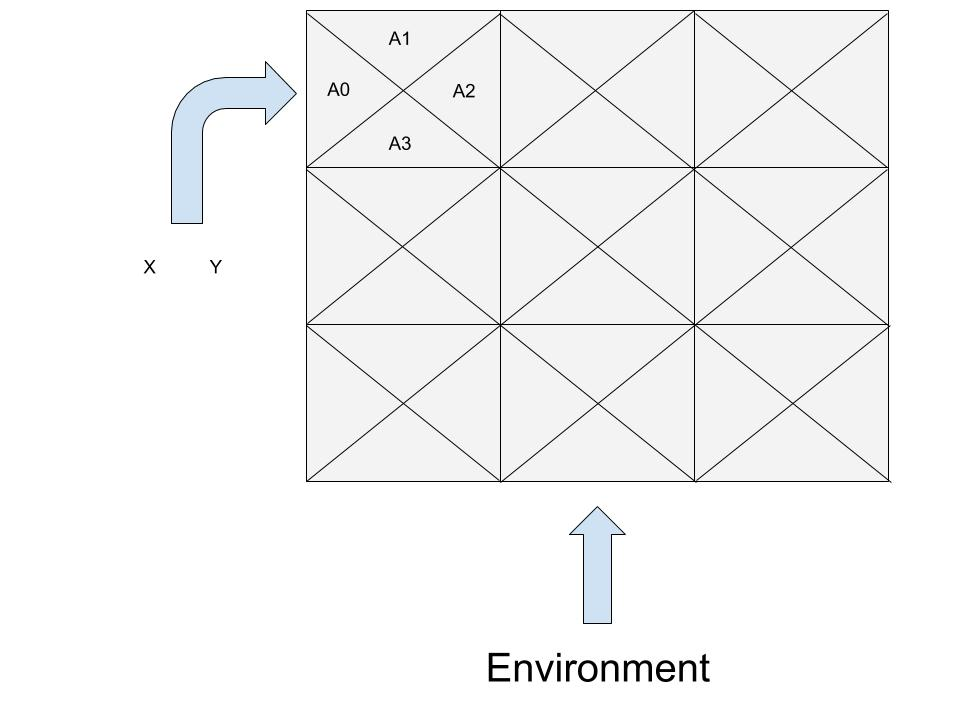
\includegraphics[width=1.4\textwidth]{assets/environment.jpg}
\end{subfigure}

\vspace{0.1in}
\label{fig:tripEmb}
\end{figure}

\end{frame}

%-------------------------------------------------------


\begin{frame}{Reinforcement Learning}{Deep Q learning}
\begin{figure}[!htb]
\centering
\begin{subfigure}[t]{0.5\linewidth}
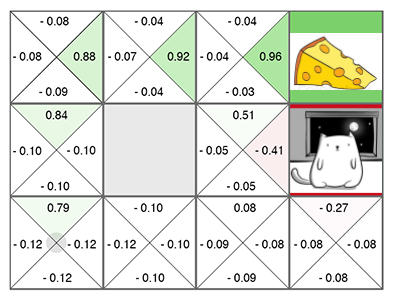
\includegraphics[width=1.3\textwidth]{assets/grid.png}
\end{subfigure}
\vspace{0.1in}
\label{fig:tripEmb}
\end{figure}
\end{frame}

%--------------------------------------------


\begin{frame}{Reinforcement Learning}{Deep Q learning}
\item What can be the best case scenario?
\pause
\begin{figure}[!htb]
\centering
\begin{subfigure}[t]{0.5\linewidth}
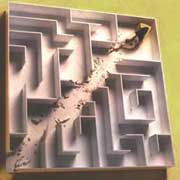
\includegraphics[width=1\textwidth]{assets/meme.jpg}
\end{subfigure}
\vspace{0.1in}
\label{fig:tripEmb}
\end{figure}
\end{frame}



%--------------------------------------------

\subsection{The approach.}

\begin{frame}{Reinforcement Learning}{Deep Q learning}
\begin{figure}[!htb]
\centering
\begin{subfigure}[t]{0.5\linewidth}
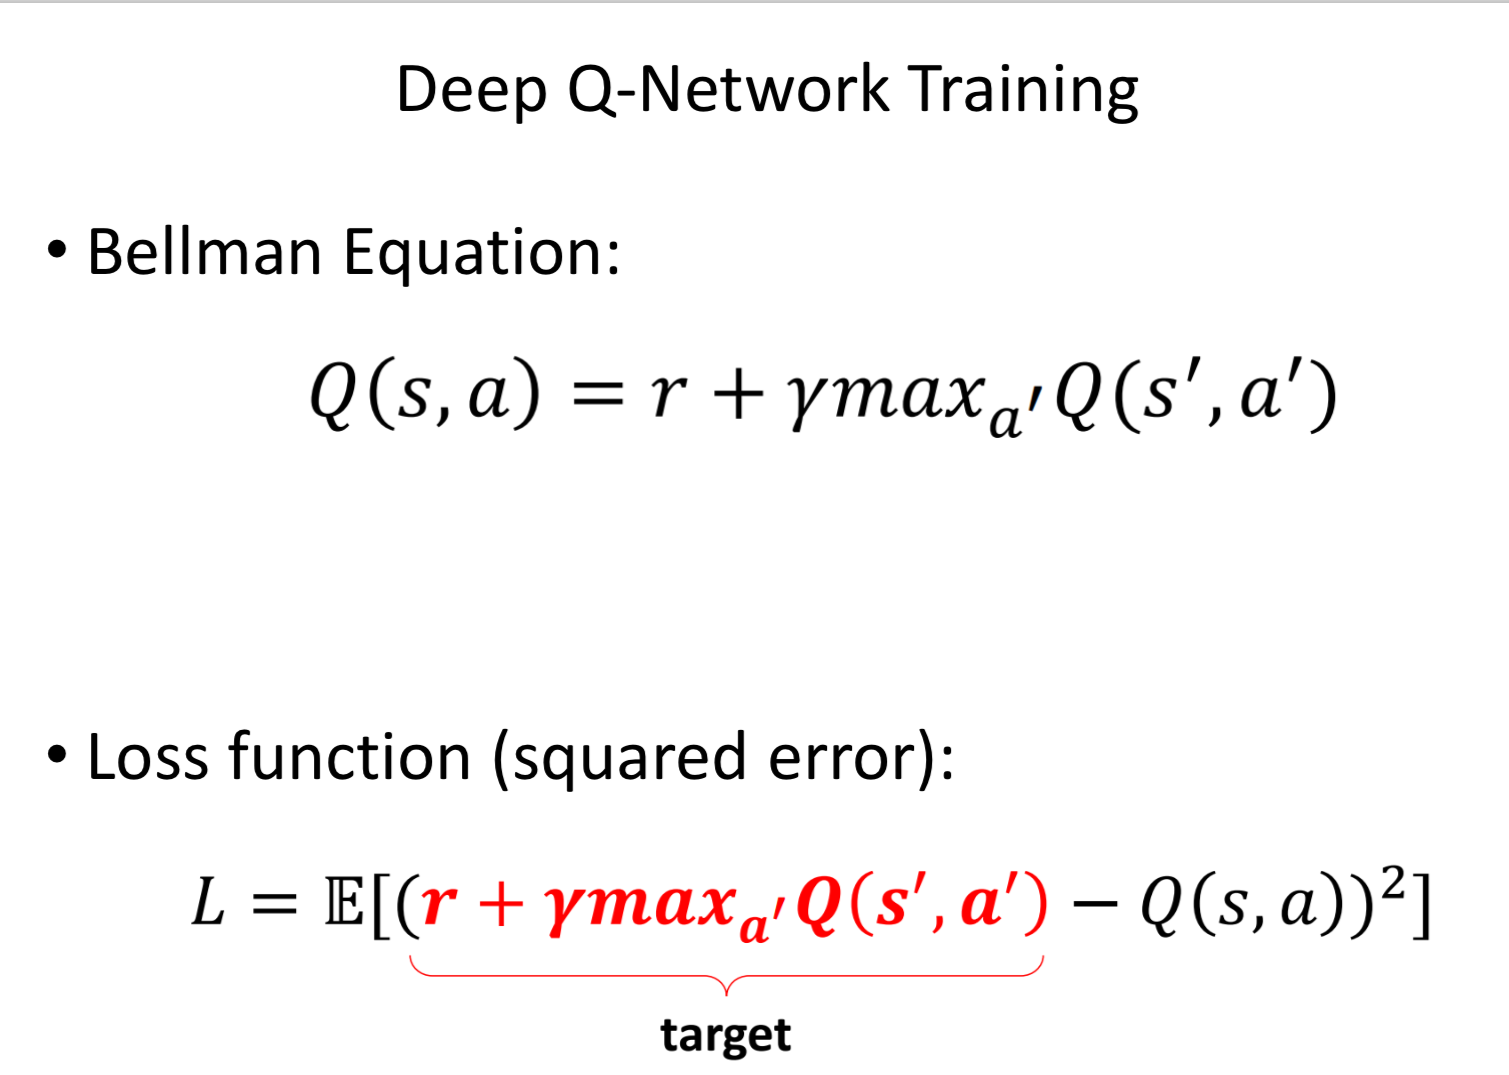
\includegraphics[width=1.5\textwidth]{assets/bellman_equation.png}
\end{subfigure}
\vspace{0.1in}
\label{fig:tripEmb}
\end{figure}
\end{frame}


%--------------------------------------------

\begin{frame}{Reinforcement Learning}{Deep Q learning}

\item Why discount the reward by gamma?
\pause
\begin{itemize}
\item So that rewards do not diverge as the time steps increase.
\end{itemize}
\pause
\begin{itemize}
\item We will be running in circles.
\end{itemize}

\end{frame}

%-------------------------------------------------------
\begin{frame}{Reinforcement Learning}{Deep Q learning}
\item Exploration!

\begin{itemize}
\item We take the optimum action but sometimes we take a random action with exploration probability $\epsilon$ so that surroundings are investigated for possible rewards.
\item We decay this $\epsilon$ over time exponentially.
\end{itemize}
% \begin{itemize}
\item $$ \epsilon = \epsilon_{min} + (\epsilon_{max} - \epsilon_{min}) * \exp^{(-\lambda * t)}  $$
% \end{itemize}

\end{frame}

%-------------------------------------------------------


\begin{frame}{Reinforcement Learning}{Deep Q learning}
\begin{itemize}
\item \textbf{Explore} - Take random actions and create a queue of (current state, action, next state, reward).     
\pause
\item \textbf{Train} - Sample from this queue and use the data to create a training data for our model to learn from. 
\begin{itemize}
\pause
\item This should be done keeping in mind that we tend to converge the bellman equation.
\pause
\item Taking a random action with a exploration probability (which decrease over time).
\pause
\item The new variables (state, action, next state, reward) acquired are pushed into the queue. 
\end{itemize}
\pause
\item \textbf{Play} - The model is tested by keeping the exploration probability as zero and stopping learning from experiences.
\end{itemize}

\end{frame}


%--------------------------------------------
%-------------------------------------------------------


\begin{frame}{Reinforcement Learning}{Deep Q learning}
\begin{figure}[!htb]
\centering
\begin{subfigure}[t]{0.5\linewidth}
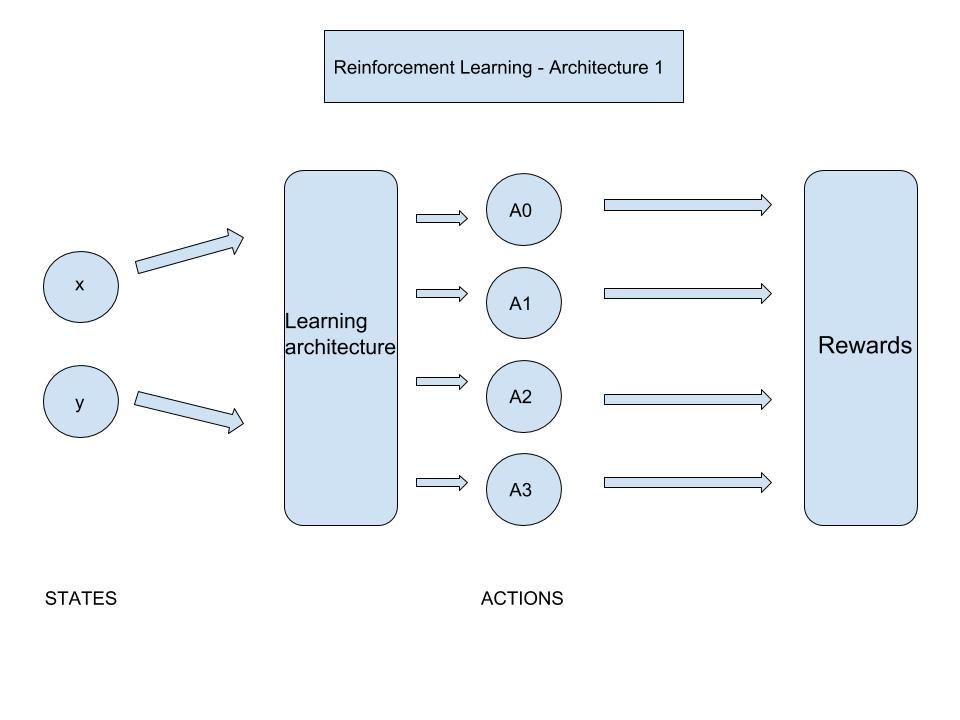
\includegraphics[width=1.3\textwidth]{assets/train.jpg}
\end{subfigure}
\begin{subfigure}[t]{0.5\linewidth}
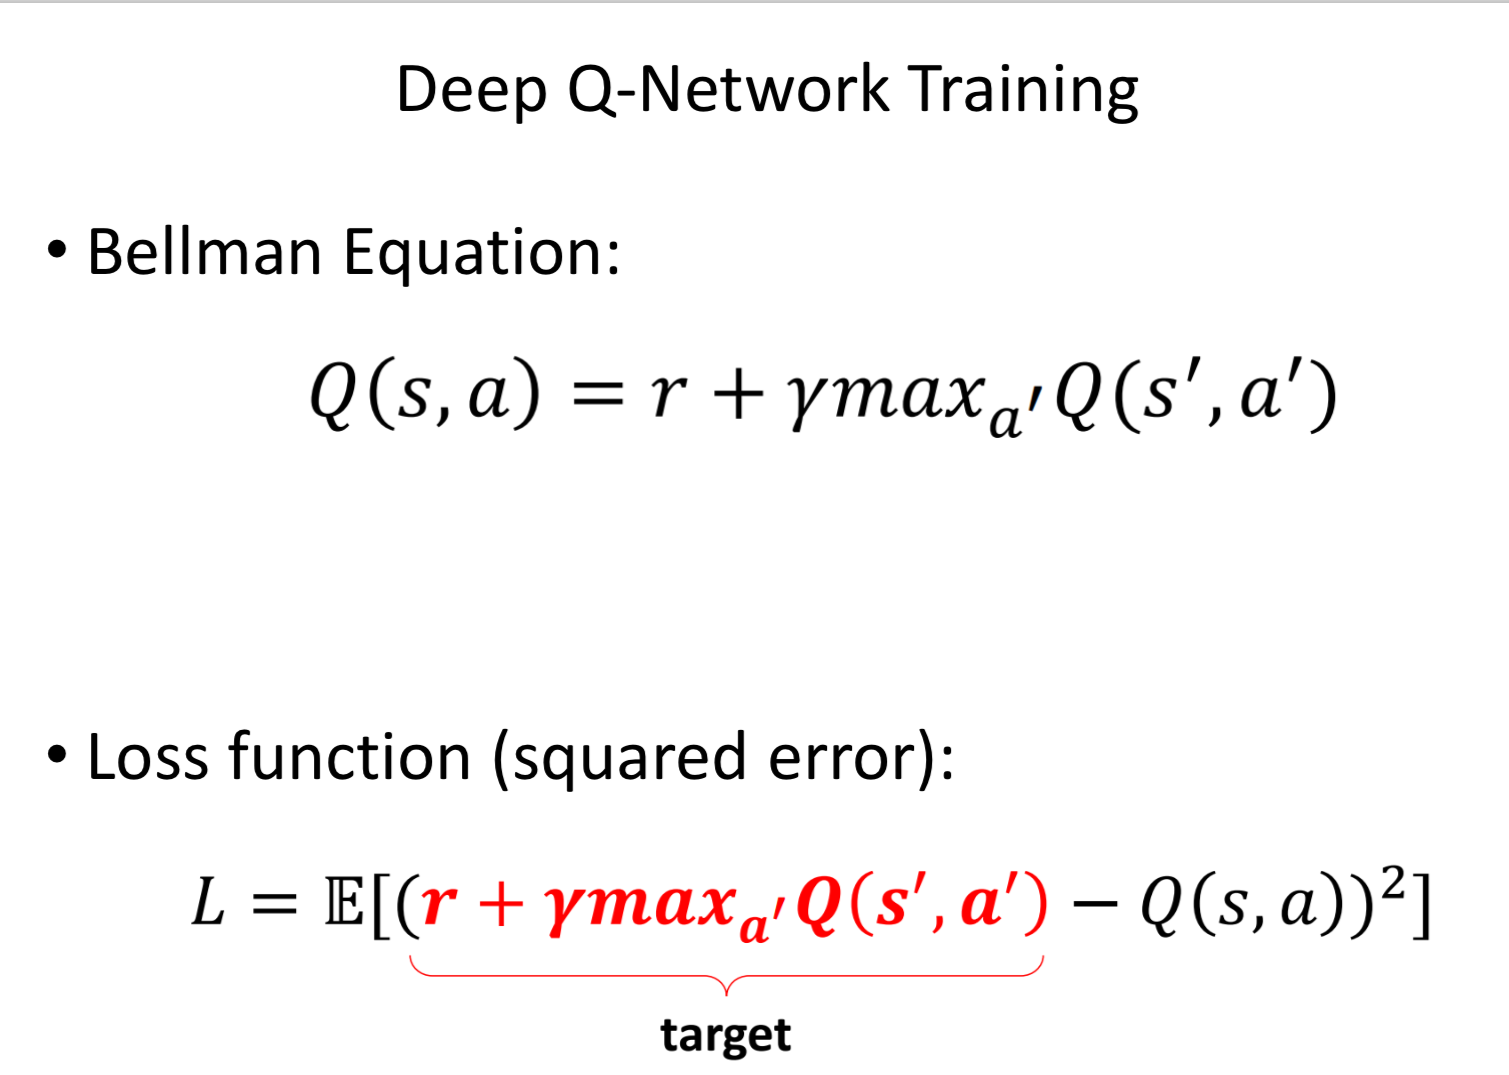
\includegraphics[width=1.3\textwidth]{assets/bellman_equation.png}
\end{subfigure}
\vspace{0.1in}
\label{fig:tripEmb}
\end{figure}
\end{frame}



%--------------------------------------------

\subsection{Flaws with DQN.}

\begin{frame}{Reinforcement Learning}{Deep Q learning}
\item There is a flaw in this approach.
\pause
\begin{itemize}
\item Our Q values shift but the target value also shifts. 
\end{itemize}
\pause
\begin{itemize}
\item Due to the max in the formula for setting targets, the network suffers from maximization bias, possibly leading to overestimation of the Q function’s value and poor performance.
\end{itemize}
 
\begin{figure}[!htb]
\centering
\begin{subfigure}[t]{0.5\linewidth}
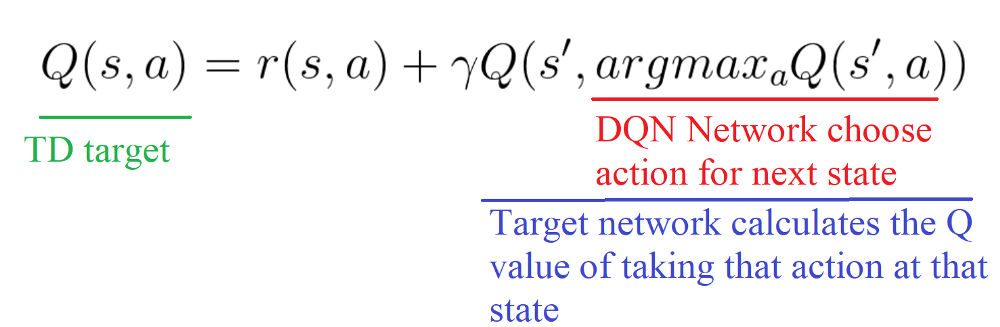
\includegraphics[width=1.5\textwidth]{assets/ddqn_equation.png}
\end{subfigure}
\vspace{0.1in}
\label{fig:tripEmb}
\end{figure}

\end{frame}


%--------------------------------------------

\begin{frame}{Reinforcement Learning}{Deep Q learning}
\item Like most all machine learning algorithms all this comes at a price.


\pause
\begin{figure}[!htb]
\centering
\begin{subfigure}[t]{0.5\linewidth}

\includegraphics[width=1.5\textwidth]{assets/meme_itsfine.png}
\end{subfigure}
\vspace{0.1in}
\label{fig:tripEmb}
\end{figure}
It uses a lot of system resources!

\end{frame}
%--------------------------------------------

\section{Practical examples}
%-------------------------------------------------------
\subsection{Gym and fromscratchtoml}
\begin{frame}{Reinforcement Learning}{Breakout}

\begin{figure}[!htb]
\centering
\begin{subfigure}[t]{0.5\linewidth}

\item \alert{Breakout by deepmind} \href{https://www.youtube.com/watch?v=TmPfTpjtdgg }{\beamergotobutton{Link}}

\end{subfigure}
\vspace{0.1in}
\label{fig:tripEmb}
\end{figure}

\end{frame}


\begin{frame}{Examples}{openAI gym and fromscratchtoml}

\item openAI gym provides an environment for your agent to learn and play around. \href{https://gym.openai.com/envs/#classic_control}{\beamergotobutton{Link}}

\item Code for machine learning algorithms from scratch -  \href{https://github.com/markroxor/fromscratchtoml}{\beamergotobutton{Link}}

\end{frame}


{\1
\begin{frame}[plain,noframenumbering]
  \finalpage{Thank You}
\end{frame}}

\end{document}